% -- Rapport
% Module : INFO606
% Année  : 2014-2015

% HADJI Monir et MOHIMONT Lucas

\documentclass[a4paper, 11pt]{article}

% -----
% ----- Preambule
% -----
\usepackage[utf8]{inputenc}
\usepackage[T1]{fontenc}
\usepackage{lmodern}
\usepackage{amsmath}
\usepackage{amssymb}
\usepackage{mathrsfs}
\usepackage{mathtools}
\usepackage[francais]{babel}
\usepackage[left=1in, right=1in, top=1.2in, bottom=1.2in]{geometry}
\usepackage{setspace}
\usepackage{layout}
\usepackage{graphicx}
\usepackage{tikz}
\usepackage{epstopdf}
\usepackage{fancyhdr}
\usepackage{lastpage}
\usepackage{hyperref}
\usepackage{parskip}
\usepackage{url}
\usepackage[ruled, vlined]{algorithm2e}

% Variables pour la page de garde
\newcommand{\nomModule}{Framework pour la visualisation d'algorithmes intéractifs}
\newcommand{\codeModule}{Info0606}
\newcommand{\respoModule}{Christophe Jaillet}
\newcommand{\authorun}{Lucas Mohimont}
\newcommand{\authordeux}{Monir Hadji}
\newcommand{\intituleProjetTP}{Projet de programmation}
\newcommand{\annee}{2014-2015}
\newcommand{\groupe}{S6O6}
\newcommand{\promo}{L3 Informatique}

% Entete / Pieds de page
\pagestyle{fancy}
\renewcommand{\headrulewidth}{0.4pt}
\renewcommand{\footrulewidth}{0pt}
\fancyhead[L]{\leftmark} \fancyhead[C]{} \fancyhead[R]{\rightmark}
\fancyfoot[L]{\groupe\ - \promo} \fancyfoot[C]{\thepage/\pageref{LastPage}} \fancyfoot[R]{\annee}

% Enlever couleur pour les liens tables matieres
\hypersetup{pdfborder={0 0 0}}

% Interligne de taille intermediaire
\onehalfspacing

% -----
% ----- Document
% -----
\begin{document}

\makeatletter

% Page de garde
\begin{titlepage}
  \centering
  \hfill 
\includegraphics[width=0.35\textwidth]{contents/urca.jpg}

  \vspace{4cm}

  \begin{flushleft}
    {\LARGE
      \bsc{\intituleProjetTP}
    }
    \vspace{0.5em}
    \hrule height 2pt
  \end{flushleft}

  \begin{flushright}
    {\large
      \textsc{\authorun} / \textsc{\authordeux}
    }
  \end{flushright}

  \vspace{2cm}

  {\Large
    \textbf{\nomModule}
  }

  \vspace{5cm}

  \begin{flushleft}
    {\large
      {\bfseries
        Responsable \codeModule:}
      \bsc{\respoModule}
    }\\
    {\large
      {\bfseries
        Responsable projet :}
      \bsc{Jean-Charles Boisson}
    }
  \end{flushleft}

  \vfill

  \large{Année \annee}
  \hfill
  \large{Groupe \groupe\ - \promo}
\end{titlepage}

\makeatother

\thispagestyle{empty}
\tableofcontents

\newpage
\thispagestyle{plain}
\setcounter{figure}{0}
\setcounter{page}{1}
\setlength{\parindent}{1cm}

\section*{Introduction}
\addcontentsline{toc}{section}{Introduction}

Ce projet a pour but de mettre à disposition des outils permettant la visualisation et l'interaction d'algorithme. Notre framework donne les composants de base permettant de créer et visualiser  des structures de données pendant l'exécution d'un algorithme.

À plusieurs étapes de la réalisation de ce projet, nous avons dû faire des choix d'utilisation de technologies en nous basant sur plusieurs contraintes. Nous verrons ces choix au fur et à mesure dans chaque section concernée. Cependant, la plupart de ces choix doivent respecter au minimum certaines contraintes communes comme la portabilité, la documentation, la maintenabilité et la récence de version.

Les besoins sont principalement liés à la visualisation. Les outils que nous devons proposer sont principalement visuels puisqu'il s'agit d'un framework accompagné d'une interface graphique.
L'application doit pouvoir offrir une interaction utilisateur. Autrement dit, nous avons besoin d'outils permettant de faire une interface graphique et interactive, avec environnement visuel en trois dimensions.
Les outils de calcul seront indispensables dans plusieurs étapes de ce projet. Principalement, des calculs algébriques pour le calcul matriciel, nous choisirons les technologies en nous basant sur des critères spécifiés dans les paragraphes en questions.

Le projet se découpe en plusieurs étapes, nous devons tout d'abord être dans la capacité à pouvoir afficher une structure, cela posera plusieurs problèmes qui seront traités un par un.
Une fois fait, le framework devra pouvoir modifier dynamiquement l'affichage afin de pouvoir visualiser - d'une certaine manière - l'exécution de notre algorithme portant sur la structure en question.
Pour finir, nous aurons à mettre en place un système de gestion d'interaction lors de l'exécution de l'algorithme, de telle sorte que l'utilisateur puisse interrompre la visualisation de l'exécution, et procéder à une modification des données (ou un choix sur la suite de l'exécution lorsqu'il y a arborescence de suite d'exécution possible), puis de pouvoir visualiser les conséquences de ses modifications des données (ou de son choix de branche d'exécution).

\newpage
\section{Choix des technologies}
\subsection{Visualisation}
Notre choix doit respecter plusieurs contraintes en plus des élémentaires évoqués plus tôt en introduction. Nous devons pouvoir afficher nos structures dans un espace en trois dimensions, il existe plusieurs librairies haut niveau permettant de faire des manipulations et de la visualisation 3D, il s'agit le plus souvent de moteur utilisé pour faire des jeux vidéos qui sont, pour la plupart, basés sur \texttt{OpenGL}. Parmi eux, nous pouvons citer Ogre3D \cite{OGRE3d} et Irrlicht Engine \cite{IRRLICHT}, qui proposent aussi toute une panoplie d'outils pour la manipulation et la visualisation d'objet 3D, puis Unity3D \cite{UNITY} qui possède toute une couche logicielle permettant de faire davantage abstraction du rendu.

Puis il existe aussi des librairies plus bas niveau comme \texttt{OpenGL} et \texttt{Direct3D} qui permettent d'interagir directement avec le pipeline graphique en définissant précisément les opérations à effectuer pour chaque sommet, cela se fait grâce à des programmes (shaders) exécutés par le GPU, ils sont écrits en langage \texttt{GLSL} pour \texttt{OpenGL}, et \texttt{HLSL} pour \texttt{Direct3D}.

Le choix entre \texttt{OpenGL} et \texttt{Direct3D} pour la partie visualisation va se faire principalement par des contraintes élémentaires définies en introduction. Notamment la portabilité. En effet \texttt{Direct3D} bien qu'équivalent à \texttt{OpenGL} est utilisable nativement seulement sur \bsc{Windows}, il peut être possible de faire tourner des applications utilisant \texttt{Direct3D} sur certaines distributions Linux, mais cela demande d'installer certaines surcouches d'émulation comme Wine. Nous préférons éviter ce genre de choses. Nous choisissons donc \texttt{OpenGL} qui est supporté par une grande partie des systèmes, dont les smartphones grâce à \texttt{OpenGL ES} (Embedded System).

\subsection{Interaction}

Concernant l'environnement graphique dans lequel nous gérerons l'interaction et l'encapsulation de \texttt{OpenGL}, nous avons à notre disposition plusieurs choix possible. Il existe : \texttt{Qt, SDL, SFML, GTKmm}. \texttt{GTKmm} et \texttt{Qt} sont des framework plus appropriés pour faire des environnements graphique. \texttt{SDL} et la \texttt{SFML} sont davantage utilisées pour de la conception 2D (jeux de plateforme en 2D, utilitaire animé, etc), et non pas pour des environnements graphiques.

Nous devons donc choisir entre \texttt{GTKmm} (qui est une interface \texttt{C++} de la librairie \texttt{GTK}) et \texttt{Qt}. À l'heure actuelle, la dernière version de \texttt{GTKmm} (version supérieure à la v3.0) n'est disponible que sur Linux et n'est pas officiellement portée sur \bsc{Windows}. \texttt{Qt} est assez reconnu concernant sa portabilité, notre choix se portera donc sur \texttt{Qt} et \texttt{OpenGL}.

\subsection{Calcul matriciel}
Lorsque nous aurons à gérer la scène en trois dimensions avec \texttt{OpenGL}, nous aurons besoin d'une librairie proposant du calcul matriciel pour la gestion de la caméra, des rotations et des translations d'objets. \texttt{Qt} propose des opérations élémentaires sur les matrices, mais nous préférons utiliser une librairie plus couramment dédié à ce genre de besoins, nous utiliserons GLM (OpenGL Mathematics) qui est complémentaire à \texttt{OpenGL} et nous permettra donc de pouvoir manipuler plus aisément les matrices permettant de gérer la caméra.

\subsection{Langage de programmation}
En partant du principe qu'il nous faudrait un langage proposant le paradigme orienté objet, nous avons le choix entre \texttt{Python}, \texttt{Java}, \texttt{C++} ou autre.

Ce projet étant surtout à but pédagogique, nous préférons utiliser le \texttt{C++}, car nous aimerions progresser dans ce langage qui propose aussi le paradigme de programmation générique avec les templates qui est l'une des facettes du langage que l'on aimerait mieux maîtriser.

\newpage
\section{Cas de la structure graphe}
Nous nous limiterons à la structure de graphe. Contrairement à des structures plus basiques comme les listes et les arbres binaires, les graphes posent plus de problèmes au niveau de leur représentations.

L'une des premières problématiques est le placement des nœuds. Les nœuds ne doivent ni se chevaucher, ni être à des distances non-uniformes par rapport à leur nœud adjacent. Nous devons donc faire en sorte que les nœuds aient un placement ordonné dans l'espace et le plus harmonieux possible. Dans toute la suite de ce rapport, le graphe d'exemple sera le suivant.

\begin{figure}[!htb]
  \begin{center}
    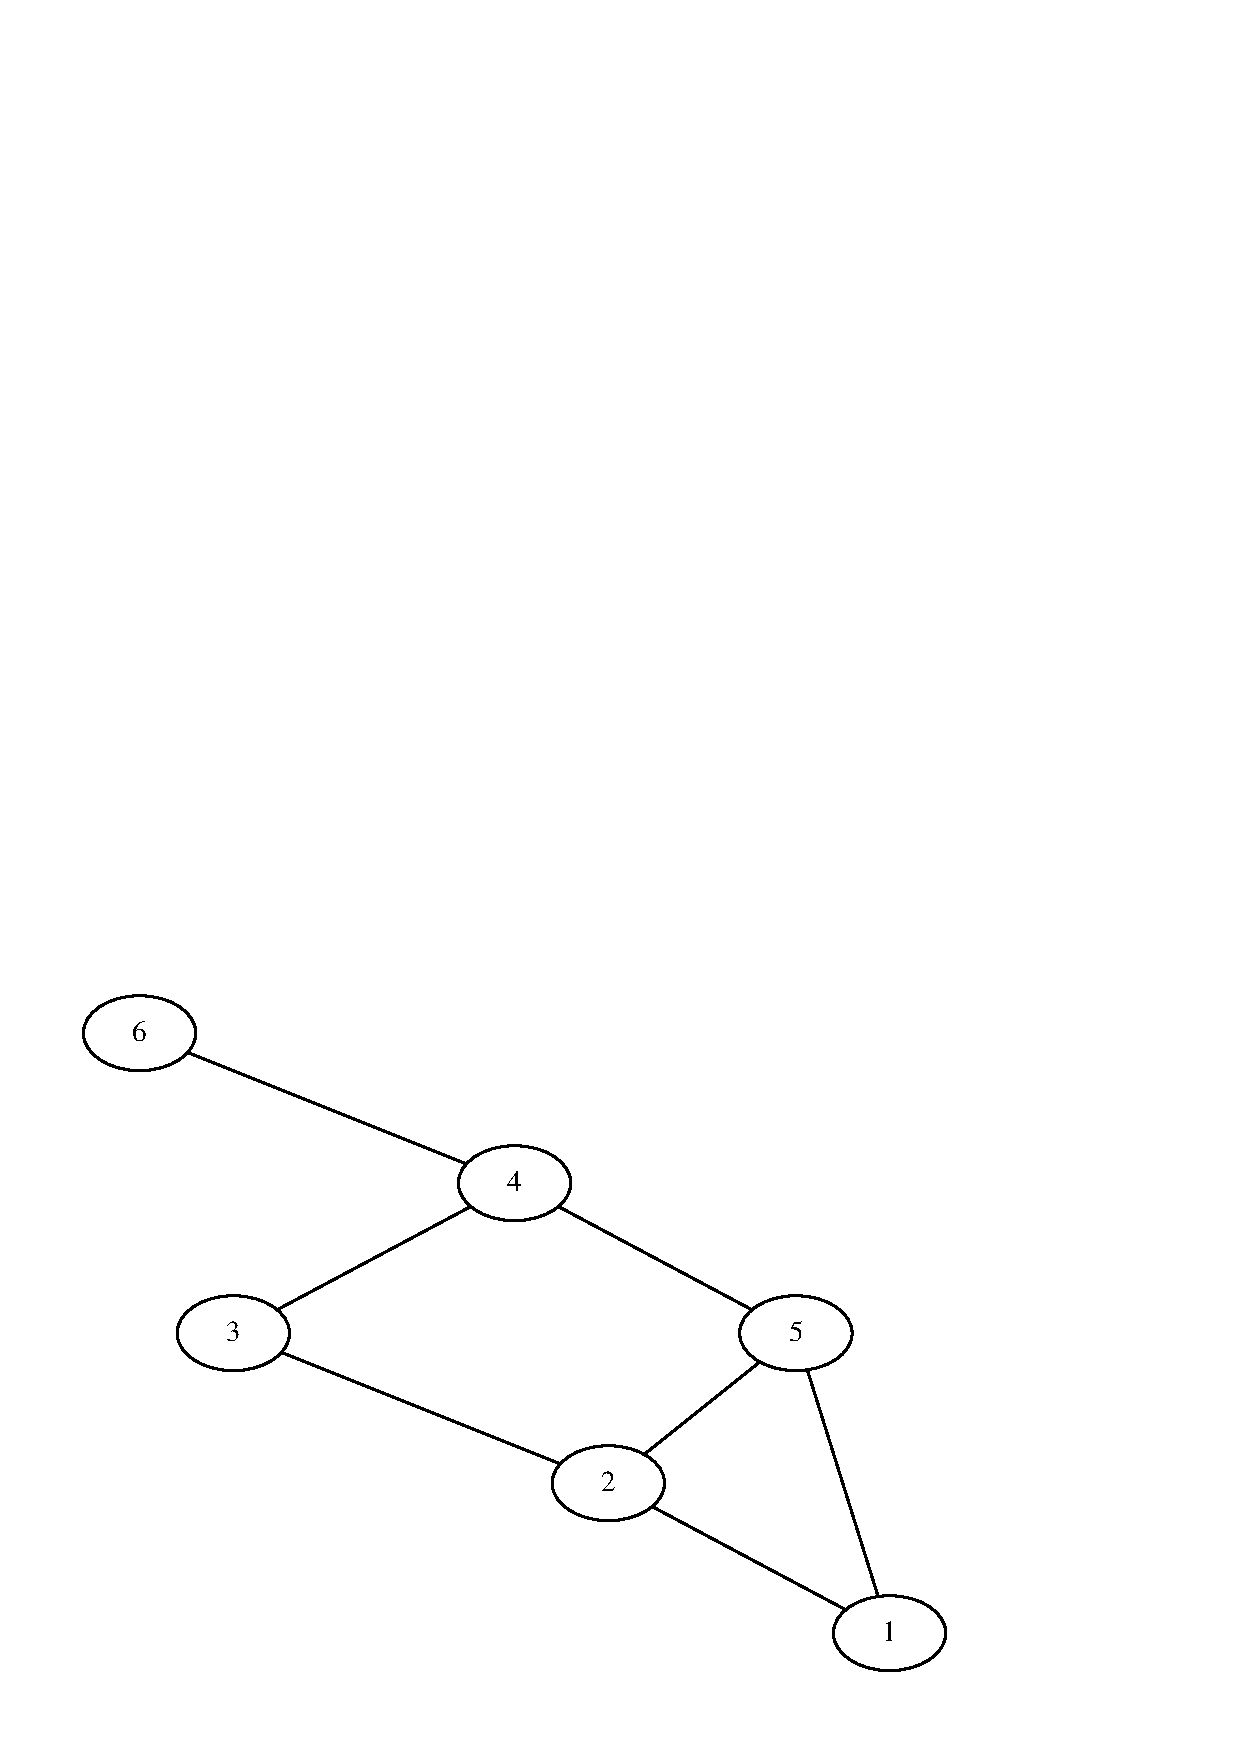
\includegraphics[scale=0.6]{contents/graphe}
  \end{center}
  \caption{Graphe G de référence pour les exemples à suivre}
  \label{fig:greference}
\end{figure}

\subsection{Placement des noeuds}
Il existe plusieurs approches mais deux en particuliers, Forced directed graph drawing \cite{forced_theorie}, et Spectral graph drawing \cite{spectral_theorie}. Les autres approches sont soit très peu documentées, soit il s'agit de variantes.

\paragraph{Force directed graph drawing}

Cette approche de placement de nœuds consiste à associer un graphe à un système physique, elle est décrite dans \cite{forced_theorie}. Des coordonnées aléatoires sont attribuées à chaque sommet. Ces coordonnées sont ensuite mises à jour en fonction des forces qui s'appliquent sur le sommet. Le calcul des forces dépend du modèle choisi. Une des analogies possibles est de considérer que les arêtes du graphe sont des ressorts. Le calcul des forces et la mise à jour des coordonnées font que le système se rapproche d'un point d'équilibre où les sommets resteront fixes et donc bien positionnés.

Pour cette approche, il existe plusieurs algorithmes présentés dans \cite{forced_theorie}. Nous nous sommes penchés sur deux algorithmes de cette approche, l'algorithme \texttt{Barycentric-Draw} et l'algorithme \texttt{Spring}. Ce dernier consiste à simuler des ressorts et est limité aux graphes de trente sommets maximum, en plus de ne pas forcement être précis, en effet, la condition d'arrêt de la boucle principale ne permet pas une solution dans tous les cas.
L'algorithme \texttt{Barycentric-Draw}  est plus précis au niveau de la condition d'arrêt, il n'est pas limité par le nombre de sommets, mais demande plus de calcul.
Avec cette approche, notre graphe ne sera pas toujours représenté avec les mêmes placements.

\paragraph{Spectral graph drawing}

Cette approche provient de \cite{spectral_theorie} et est décrite dans la section 3.1.
Nous devons utiliser la représentation par matrice Laplacienne. Puis à partir de calcul de valeurs et vecteurs propres sur cette matrice laplacienne, nous pouvons obtenir des valeurs permettant un placement harmonieux des nœuds dans l'espace considéré. Il s'agit de cette approche que nous allons développer dans la suite de ce rapport.

\subsubsection{Représentation matricielle}
Soit un graphe $G=(V,E)$ avec $V$ l'ensemble des nœuds, et $E$ l'ensemble des arêtes.\\
Notation:
\begin{itemize}
\item[-] $L^G$ la matrice Laplacienne du graphe $G$
\item[-] $L^G_{ij}$ le scalaire à la ligne $i$ et colonne $j$ de la matrice $L^G$.
\item[-] $deg(i)$ le degré du nœud $i$.
\item[-] $w_{ij}$ le poids de l'arête $(i,j)$.
\end{itemize}

\begin{equation}
  w_{ij} =
  \left\{
  \begin{array}{r l l}
    0 &si& (i,j) \notin E \\
    \text{le poids de l'arête } (i,j) &si& i \neq j \text{ et } (i,j) \in E \\
  \end{array}
  \right.
\end{equation}

Nous avons la définition $(1)$ dans le cas où $G$ est non-pondéré et non-orienté. La définition $(2)$ dans le cas où $G$ est pondéré et orienté.\\

\begin{equation}
  L^G_{ij} =
  \left\{
  \begin{array}{r l l}
    deg(i) &si& i = j \\
    -1 &si& i \neq j \text{ et } (i,j) \in E \\
    0 &sinon&
  \end{array}
  \right.
\end{equation}

\begin{equation}
  L^G_{ij} =
  \left\{
  \begin{array}{r l l}
    deg(i) &si& i = j \\
    -w_{ij} &si& i \neq j\\
  \end{array}
  \right.
\end{equation}

\paragraph{Application au graphe de référence G}

Ainsi, pour le graphe G dont la représentation est visible en Fig.~\ref{fig:greference}, nous obtenons la matrice laplacienne suivante.

\[
L^G =
\begin{pmatrix*}[r]
  2 & -1 & 0 & 0 & -1 & 0\  \\
  -1 & 3 & -1 & 0 & -1 & 0\  \\
  0 & -1 & 2 & -1 & 0 & 0\  \\
  0 & 0 & -1 & 3 & -1 & -1\  \\
  -1 & -1 & 0 & -1 & 3 & 0\  \\
  0 & 0 & 0 & -1 & 0 & 1\
\end{pmatrix*}
\]

La matrice $L^G$ est toujours symétrique. Le fait de savoir que cette matrice est forcement symétrique nous servira par la suite, car cela nous permettra d'améliorer le temps de calcul en spécifiant aux fonctions en questions lors du calcul des valeurs propres que notre matrice est symétrique.

\subparagraph{Preuve}
On note $I$ la matrice d'incidence de $L^G$. La matrice $L^G$ peut être obtenu par le produit de $I$ et de sa transposée $^tI$.
Or, le produit d'une matrice par sa transposée est forcement symétrique.\footnote{$^t(^tA \cdot A) =\ ^tA\ \cdot \ ^t(^tA) =\ ^tA \cdot A$ \\ une matrice égale à sa transposée est symétrique.}

\subsubsection{Approche intuitive}
\paragraph{À Noter}
Le but de cette section est principalement d'avoir une approche intuitive concernant la description symbolique des vecteurs solutions que nous cherchons. Cette section ne donne pas le lien entre la procédure en pratique et la description mathématique des vecteurs solutions que nous voulons. Pour cela, il aurait fallu bien comprendre le cheminement et la démonstration mathématique décrite dans \cite{spectral_theorie}. Cependant, nous n'avons ni les bagages techniques suffisants, ni eu le temps de nous pencher davantage sur la compréhension complète de cette approche. Il nous semblait plus pertinent - dans un premier temps - de nous focaliser sur la mise en pratique de cette méthode, décrite dans \cite{spectral_pratique}, plutôt que de nous pencher sur une compréhension profonde du fonctionnement intrinsèque de cette approche.


Nous cherchons $x^1,...,x^p$ qui sont les vecteurs correspondants aux coordonnées voulues dans un espace de dimension $p$. Ainsi $x^1(i)$ correspond à la coordonnée du nœud $i$ sur le premier axe. Et $x^3(i)$ correspond également à la coordonnée du nœud $i$ mais sur le troisième axe (troisième axe qui est l'axe usuel $z$ si nous sommes dans un espace à trois dimensions, i.e $p=3$).

La notation suivante nous renseigne le carré de la norme euclidienne entre les nœuds $i$ et $j$ dans un espace de dimension $p$.

\[
d_{ij}^{2} = \sum_{k=1}^{p} (x^k(i) - x^k(j))^{2}
\]

Plaçons-nous dans le cas où nous souhaitons obtenir les coordonnées de placement des nœuds dans un espace à trois dimensions, donc avec $p=3$. Nous voulons donc les vecteurs $x^1$, $x^2$ et $x^3$ (chacun appartenant à $\mathbb{R}^{n}$ avec $n$ le nombre de nœuds) avec la relation suivante.

\[
\min_{x^1, x^2, x^3} E(x^1, x^2, x^3) = \frac{\sum_{(i,j)\in E} w_{ij}d_{ij}^2 }{ \sum_{i<j} d_{ij}^2}
\]

Les vecteurs solutions $x^1$, $x^2$ et $x^3$ correspondent aux vecteurs obtenus en minimisant la fraction de droite. Cette dernière a un numérateur représentant la longueur moyenne des arêtes du graphe, le dénominateur répresente la distance moyenne entre chaque nœud. Cette fraction doit être minimale. Pour cela il faut minimiser le numérateur de telle sorte que la longueur moyenne des arêtes soit la plus petite possible. Puis, il faut maximiser le dénominateur de telle sorte que la distance entre chaque nœud soit maximale (de manière relative au numérateur) ce qui va créer un équilibre entre ces deux métriques. En effet, plus la fraction sera minimale, et plus nous aurons une longueur d'arête minimale et une distance entre chaque nœud le plus espacé possible.

Le calcul est fait en utilisant des contraintes, par exemple avec $Var(x^1) = Var(x^2) = Var(x^3) = c$ avec $c$ une constante. Ainsi le calcul sera fait en étant contraint d'avoir une variance égale et constante sur tous les axes, grâce à cette contrainte nous auront des nœuds avec une dispersion équitable sur les axes respectifs.

\subsubsection{Procédure en pratique}

La mise en pratique de cette méthode va se faire à partir de calcul de valeurs et vecteur propre associé à $L^G$. $n$ représente le nombre de nœud du graphe.

\begin{algorithm}[H]
  \KwIn{$L^G$ : Matrice laplacienne du graphe $G$}
  \KwData{\texttt{val\_vec\_propre} : Tableau associatif <valeur propre|vecteur propre> de $L^G$ dans l'ordre croissant des valeurs propres. \texttt{val\_vec\_propre($i$, $j$) représente la valeur $i$ du vecteur propre associé à la valeur propre $j$}}
  \KwResult{\texttt{X,Y,Z} : Les trois vecteurs de dimension $n$ contenant les coordonnées de nœuds, \texttt{X(i)} est la position sur l'axe \texttt{X} du nœud \texttt{i}}

  \emph{Calcul des valeurs propres et vecteurs propre associés}
  \newline
  \For{$i$ allant de $1$ à $n$}
      {
        \texttt{X($i$)} $\longleftarrow$ \texttt{val\_vec\_propre($i$, 2)}\;
        \texttt{Y($i$)} $\longleftarrow$ \texttt{val\_vec\_propre($i$, 3)}\;
        \texttt{Z($i$)} $\longleftarrow$ \texttt{val\_vec\_propre($i$, 4)}\;
      }
      \caption{Placement de nœud (Spectral Graph Drawing)}
\end{algorithm}

Le nombre de valeurs propres est renseigné par le degré du polynôme caractéristique $P_{L^G}(\lambda)$ qui est égale au déterminant de la matrice $L^G$ auquel on soustrait $\lambda$ à la diagonale. Ce déterminant ne peut pas avoir un degré supérieur à la dimension de la matrice. Par conséquent, pour un graphe de $n$ nœuds, nous ne pourrons pas avoir plus de $n$ valeurs propres, et donc nous aurons au maximum une représentation sur $n-1$ dimensions.

Autrement dit, pour un graphe de trois nœuds, nous aurons au maximum trois valeurs propres, nous pourrons donc représenter ce graphe sur seulement deux dimensions. Remarquons que cela ne pose pas de problème puisque trois points sont forcément présent dans un plan commun, nous pouvons donc représenter un graphe de trois nœuds dans un plan.

\paragraph{Application au graphe de référence G}
Rappelons tout d'abord que $G$ est un graphe de six nœuds ($|V| = 6$), sa laplacienne $L^G$ sera donc carrée et de taille (6,6). Ainsi, $P_{L^G}(\lambda)$ a un degré au maximum égale à 6, donc 6 valeurs propres au maximum.

Tableau rassemblant les résultats de calculs de valeurs et vecteur propre associé pour la matrice $L^G$.

\texttt{
  \begin{tabular}{|c||r|r|r|r|r|}
    \hline
    Valeur propre & -3.7007e-17 & 0.7215 & 1.6825 & 2.9999 & 3.7046 \\
    \hline
    \multicolumn{6}{c}{} \\
    \hline
    Nœuds & \multicolumn{5}{c|}{Les vecteurs propres associés} \\
    \hline
    1 & -0.40824 & 0.41486 & -0.50529 & 0.28867 & -0.56702 \\
    \hline
    2 & -0.40824 & 0.30944 & 0.04026 & 0.28867 & 0.65812 \\
    \hline
    3 & -0.40824 & 0.06923 & 0.75901 & 0.28867 & -0.20514 \\
    \hline
    4 & -0.40824 & -0.22093 & 0.20066 & -0.57735 & -0.30843 \\
    \hline
    5 & -0.40824 & 0.22093 & -0.20066 & -0.57735 & 0.30843 \\
    \hline
    6 & -0.40824 & -0.79354 & -0.29398 & 0.28867 & 0.11403 \\
    \hline
  \end{tabular}
}

Selon l'algorithme de placement de nœuds : les éléments du vecteur \texttt{X} seront ceux du vecteur propre correspondant à la valeur propre \texttt{0.7215}), ceux du vecteur \texttt{Y} seront ceux de la colonne juste après, puis la cinquième colonne pour le vecteur \texttt{Z}.\\
Ainsi, les coordonnées \texttt{(x,y,z)} du troisième nœud seront \texttt{(0.06923 ; 0.75901 ; 0.28867)}.
La figure.~\ref{fig:G3D} suivante correspond au positionnement des points à partir des coordonnées calculées précedemment.\\
Rappelons qu'il s'agit donc du positionnement des nœuds du graphe G de référence représenté à la figure.~\ref{fig:greference}

\begin{figure}[ht]
  \begin{center}
    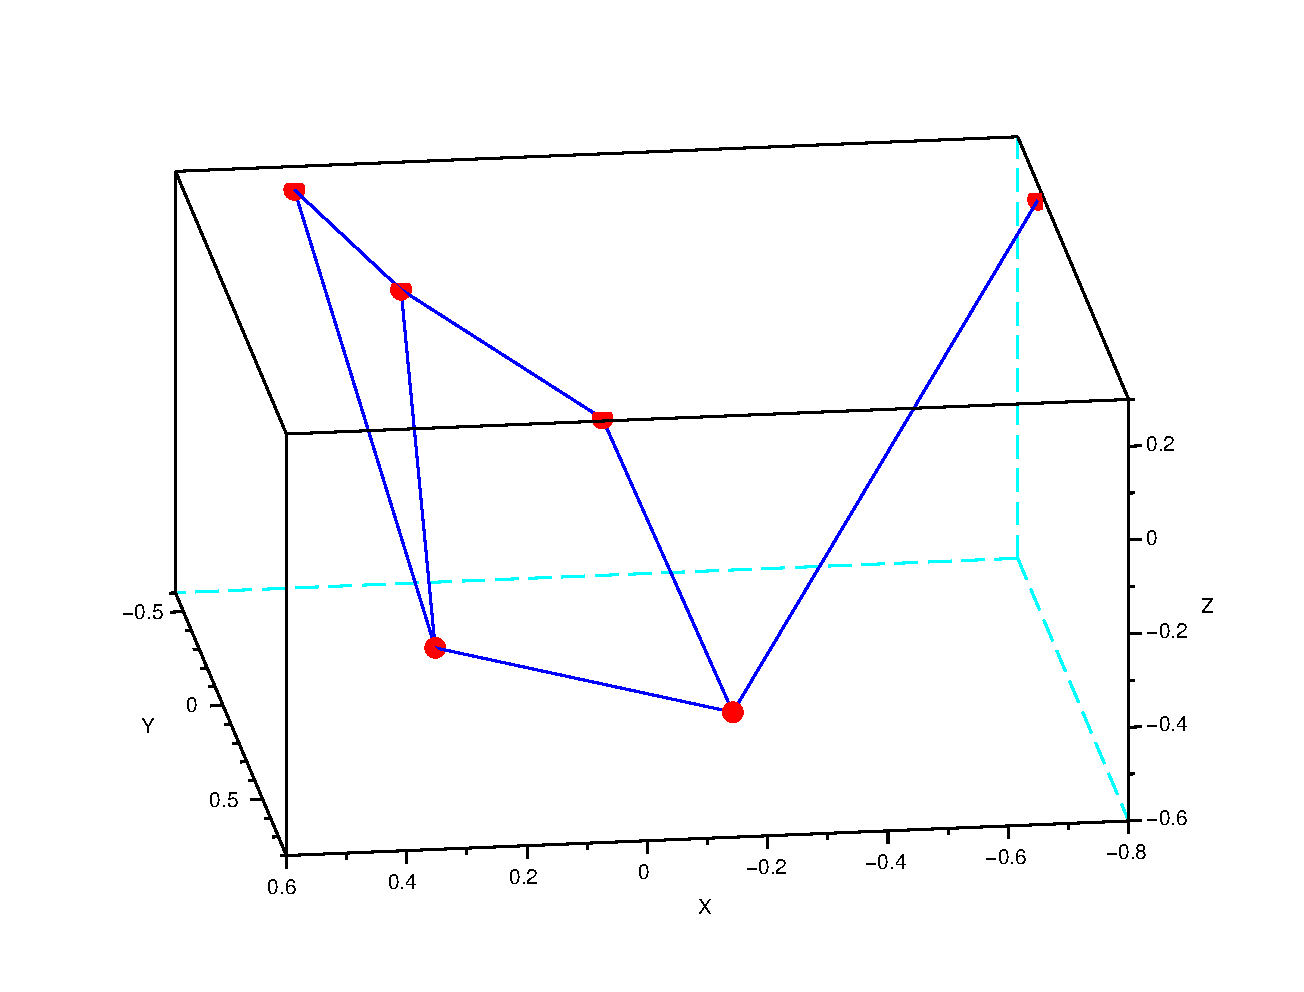
\includegraphics[scale=0.4]{contents/grefsci}
  \end{center}
  \caption{Représentation 3D du graphe de référence sur Scilab}
  \label{fig:G3D}
\end{figure}

Désormais, nous aimerions integrer cette approche de placement de nœuds dans notre application en utilisant des technologies choisient de manière pertinente.

\subsubsection{Technologie}

Il existe plusieurs algorithmes et variante pour le calcul de valeur/vecteur propre. Ceux-ci sont relativement plus ou moins adaptés selon nos contraintes et nos données de départ. En pratique, nous connaissons le nombre de valeur et vecteur propre que nous voulons calculer, il s'agit d'au maximum quatre, en prenant les vecteurs propres correspondant aux trois plus grandes valeur propres parmi les quatre. Nous savons aussi que pour l'heure, nous nous sommes focaliser sur des graphes non-orientés, donc notre matrice laplacienne est symétrique. Pour le calcul de valeurs et vecteurs propres, il existe l'algorithme de \bsc{Lanczos}, ainsi que l'algorithme LOBPCG (Locally Optimal Block Preconditioned Conjugate Gradient). Ces deux algorithmes sont apparemment les plus courants. Que nous utilisions l'un ou l'autre, nous n'aurons certainement pas de différences très significatives en pratique dans notre contexte. Cependant, il est intéressant de noter que l'algorithme LOBPCG semble être plus approprié dans notre cas. En effet, l'algorithme de Lanczos semble plus adapté lorsque l'on cherche à calculer les plus grandes valeurs propres d'une matrice le plus rapidement possible. De plus, d'après \cite{lobpcg}, l'algorithme LOBPCG serait plus efficace lorsque l'on cherche à aussi calculer les vecteurs propres associés.

Plusieurs librairies proposent une implémentation de ce genre d'algorithmes, mais certains sont beaucoup trop exotiques, accompagné d'une documentation qui nous semble assez hasardeuse et difficile d'accès (Hypre et PETSc qui proposent une API vers l'implémentation BLOPEX \cite{BLOPEX} qui implémente des algorithmes spécifiques aux calculs de valeurs/vecteurs propres), et d'autres sont beaucoup trop dense (trilinos \cite{TRILINOS}) bien que complet, mais beaucoup trop lourd à utiliser dans notre contexte. Nous avons donc au final choisis d'utiliser une librairie générique : \cite{GSL} (GNU Scientific Library) qui nous propose une implémentation classique de l'algorithme de Lanczos. Cette librairie est plus facile d'accès et nous permettra donc de programmer plus facilement cette partie externe consistant à placer nos nœuds. Une présence plus forte de calculs de valeurs et vecteurs propres nous aura certainement poussés vers un autre choix.

\subsection{Rendu}

Dans la première partie, nous avons argumenté notre choix pour l'utilisation de \texttt{OpenGL} version supérieure à 3.3 pour la visualisation. Dans cette partie, nous aborderons donc la façon dont nous avons choisi de gérer les principaux composants permettant une visualisation de nos structures de données. Tout d'abord, nous verrons comment afficher les arêtes d'un graphe, puis nous verrons la gestion de la camera, puis l'affichage des nœuds, et enfin du texte pour les labels et identifiants de cellule de données.

\subsubsection{Arêtes}

Dans la partie précédente, nous avons résolu le problème de placement des nœuds, nous avons donc l'algorithme nous permettant d'obtenir les coordonnées des nœuds d'un graphe dans un espace en trois dimensions. Nous considérons donc dans cette partie que les coordonnées des nœuds ont été calculées grâce à la méthode expliquée plus tôt. Pour le rendu des arêtes, nous utiliserons un vertex shader et un fragment shader élémentaires qui gère seulement la couleur et les coordonnées de position, cela est suffisant pour les arêtes.

Dans un premier temps, nous aimerions avoir un affichage de nos arêtes. Pour cela, nous stockons les données graphiques des sommets dans la VRAM\footnote{Ou dans de la DRAM dédiée à la vidéo.\\En effet, dans le cas d'un processeur Intel récent, les VBO et VAO sont stockés dans une partie (45\%) dédiée de la DRAM, source \cite{intel} slide 26} grâce à un Vertex Buffer Objects (VBO). Ces données peuvent être multiples, nous avons bien sûr les coordonnées des sommets, mais nous pouvons rajouter d'autres données, comme des couleurs RGB, les normales aux sommets pour la gestion des lumières, les coordonnées de textures (uv map). Chaque groupe de données relatif à un sommet est associé à un identifiant de sommet. Nous pouvons par la suite faire référence aux mêmes données de sommets grâce à ce simple identifiant. Ainsi, lors de la définition des arêtes et que nous voulons faire référence au même sommet à plusieurs reprises, il nous suffit de faire référence à cet identifiant, et nul besoin de stocker inutilement toutes les données relatives au sommet.

En pratique, nous utilisons un Element Buffer Object (EBO) qui va nous permettre de stocker les arêtes de la forme suivante : \texttt{ \{ 3 , 1 , 1 , 2 , 3 , 2 \} } qui signifie le tracer des arêtes \texttt{(3,1)}, \texttt{(1,2)} et \texttt{(3,2)}. Nous affichons ces arêtes avec l'appel à la primitive \texttt{glDrawElements}, en spécifiant qu'il s'agit d'un rendu d'arêtes.

Nous aboutissons à la figure .~\ref{fig:gledge} qui représente le graphe de référence dans notre application \texttt{OpenGL}. Cependant, un rendu du graphe tel quel ne peut pas du tout convenir pour la visualisation de la grande majorité des algorithmes. En effet, rien qu'un simple parcours en profondeur serait difficilement visualisable sans avoir de véritable nœuds de graphe. Ici, nous ne sommes en présence que de simple intersection d'arêtes faisant office de nœuds.

\begin{figure}[ht]
  \begin{center}
    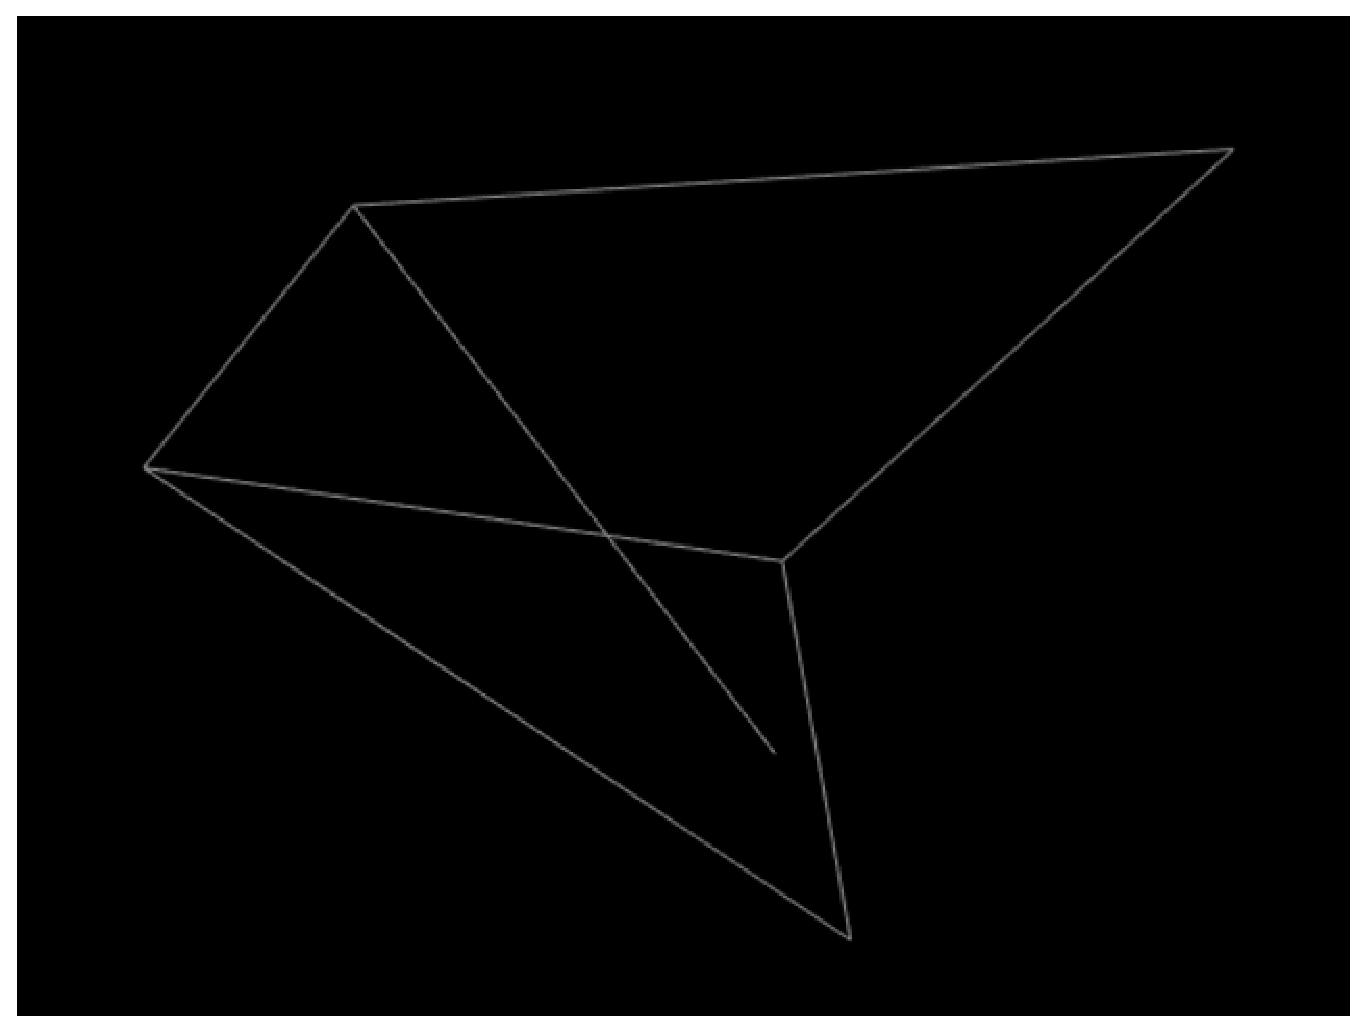
\includegraphics[scale=0.4]{contents/edge}
  \end{center}
  \caption{Arêtes du graphe de référence avec \texttt{OpenGL}}
  \label{fig:gledge}
\end{figure}

\subsubsection{Nœuds}
%\subsubsection{Structure et représentation}
\paragraph{Structure}

Cette partie a pour but la visualisation correcte de nœuds de graphe. Pour cela, nous allons introduire un typage de cellule de données (ici, il s'agit de nœuds, mais cela pourrait être une cellule de liste ou de tableau), et associer un ensemble de données (géré par une structure) à chaque type de nœuds grâce à un tableau associatif (\texttt{std::map} dans notre cas) dans la classe gérant la scène \texttt{OpenGL}.

Dans la classe gérant le rendu de la scène, nous avons donc un tableau associatif qui vient associer un type \texttt{enum} à une structure de donnée contenant plusieurs informations lié au rendu. Cette structure \texttt{DataNode} contient un vecteur RGB renseignant la couleur de la lumière à projeter sur le modèle, puis un vecteur de paire, qui associe un vertex arrays objects aux données 3D à afficher. Bien que le vertex arrays objects soit un buffer mémoire contenant les opérations à effectuer durant le rendu (opérations comme verrouillage de VBO et de shaders etc) sur des données déjà renseigné en mémoire grâce aux VBO, il est tout de même nécessaire d'associer le VAO aux données 3D à afficher, car il y a besoin de renseigner certaines informations explicitement lors de l'appel à la primitive \texttt{glDrawElements} permettant le rendu.

Les types de données sont représentés par une énumération. Nous sommes en présence d'une classe \texttt{Structure}, cette classe va gérer le placement des éléments de la structure (algorithme présenté dans la section précédente dans le cas d'un graphe), ainsi qu'un vecteur (\texttt{std::vector} dans notre cas) de type \texttt{enum} en valeur, et dont la clef correspond à l'identifiant du nœud. Ainsi, lors du rendu, nous pourrons parcourir ce vecteur, et savoir comment représenter le nœud courant grâce au tableau associatif présent dans la classe gérant le rendu de la scène permettant de récupérer les données de représentation (structure \texttt{DataNode}) à partir du type enum.

Le contenu du tableau associatif associant le type enum aux données est chargé en mémoire lors de l'initialisation de la scène de rendu. Dans la fonction d'initialisation du widget \texttt{OpenGL} (\texttt{initializeGL}), nous faisons appel à une lambda fonction se chargeant d'ajouter un nouveau champs dans le tableau associatif, nous passons en paramètre le type enum, puis les données de représentation associé à ce type. Par conséquent, les données de visualisation sont stocké en mémoire dès la création de la scène, et ce, pour tous les types enum.

\paragraph{Représentation}

Nous aimerions avoir une représentation des nœuds à partir d'un modèle en trois dimensions, comme une sphère, un cube, ou tout autre forme élémentaire concevable dans une application d'édition de modèle 3D comme \bsc{Google Sketchup} ou logiciels plus évolué comme \bsc{Autodesk 3DS Max}, \bsc{Autodesk Maya} ou même \bsc{Blender}.

Pour cela, nous devons utiliser un format de fichier permettant l'utilisation de modèle 3D, il en existe plusieurs. Parmi eux, nous pouvons citer le format 3DS Max file \texttt{(.3ds)}, le format Collada \texttt{(.dae)}, le format Wavefront OBJ \texttt{(.obj)}, et le format Python Lex\&Yacc \texttt{(.ply)}, il en existe plusieurs autres.

Le format Wavefront OBJ et Python Lex\&Yacc sont des formats très simpliste et assez vieux, ceux-ci peuvent gérer plusieurs types d'informations parmi les plus rudimentaires, comme les coordonnées de sommets, les coordonnées de textures (uv map) et les normales aux sommets.

Le format 3DS Max file, il s'agit d'un format binaire développé par Autodesk qui est, à l'origine, utilisé par leur logiciel de modélisation \bsc{Autodesk 3DS Max}. Des analyseurs syntaxiques et API de ce format sont, pour la plupart, payant. Ce format peut contenir plusieurs types d'informations dont certains rudimentaires, mais aussi d'autres types d'informations moins courants, comme les couleurs diffuses et ambiantes ainsi que la lumière spéculaire de la scène et d'autres données relative à la gestion des lumières, ainsi que plusieurs autres données que nous n'utiliserons pas dans nos modèles (données relatives aux squelettes pour l'animation squeletalle de personnage en 3D, ce qui est inutile dans notre contexte). Ce format peut contenir quasiment tous types d'informations relatives à un modèle 3D. Cependant, ce format est binaire, et les analyseurs/chargeur de ce type de fichier sont peu nombreux et parfois payant.

Le format Collada, abréviation de ''Collaborative Design Activity''. Il s'agit de base d'un format XML ayant pour but l'échange de fichiers 3D. Ce format d'échange a été développé de base pour permettre l'exportation de modèle 3D conçu dans un logiciel de modélisation A, et qu'il puisse ensuite être importable dans un autre logiciel de modélisation B, cela était très utile lorsque les logiciels de modélisation utilisaient des formats de fichiers propriétaires et fermés, il était donc difficile d'avoir des convertisseurs pour passer d'un logiciel à un autre pour la conception d'un modèle 3D. Il est possible d'utiliser ce format d'échange de fichiers 3D comme un conteneur de modèle 3D, et donc directement analyser ce type de format de fichier pour le charger et l'afficher ensuite. Nous utiliserons ce format de fichier, car il existe de nombreux analyseur/chargeur sous forme d'API, et il s'agit aussi d'un format XML qui est donc plus facilement manipulable rapidement qu'un format binaire. Nous n'écrirons pas notre propre analyseur/chargeur de fichier Collada car cela serait assez fastidieux. Ce format peut contenir quasiment autant de type d'informations que le type 3DS Max file. Les principaux avantages du format Collada sont le format XML et les nombreux analyseur/chargeur disponibles en open source et libre de droits, nous utiliserons donc ce format.

Nous utilisons une API open source pour gérer l'analyse et le chargement des modèles 3D au format Collada. Celle-ci permet de récupérer une structure contenant toutes les informations relatives au modèle passé sous forme de fichier. Cette structure offerte par l'API est ensuite mise en mémoire dans des VBO, puis ces derniers sont mis à disposition dans la structure \texttt{DataNode}, et donc récupérable par la suite grâce au tableau associatif permettant de récupérer les informations du modèle à partir du type enum lors du rendu. Le vertex shader et le fragment shader utilisés seront ceux qui ont été codé par les auteurs de l'API que nous utiliserons, le vertex shaders se contente simplement de positionner les coordonnées de sommets sans aucune modification de position, puis de transmettre au fragment shaders les normales aux sommets, quant au fragment shader, celui-ci va projeter la lumière diffuse de couleur décidé dans le programme, ainsi que la lumière ambiante et spéculaire.

\begin{figure}[h]
  \begin{center}
    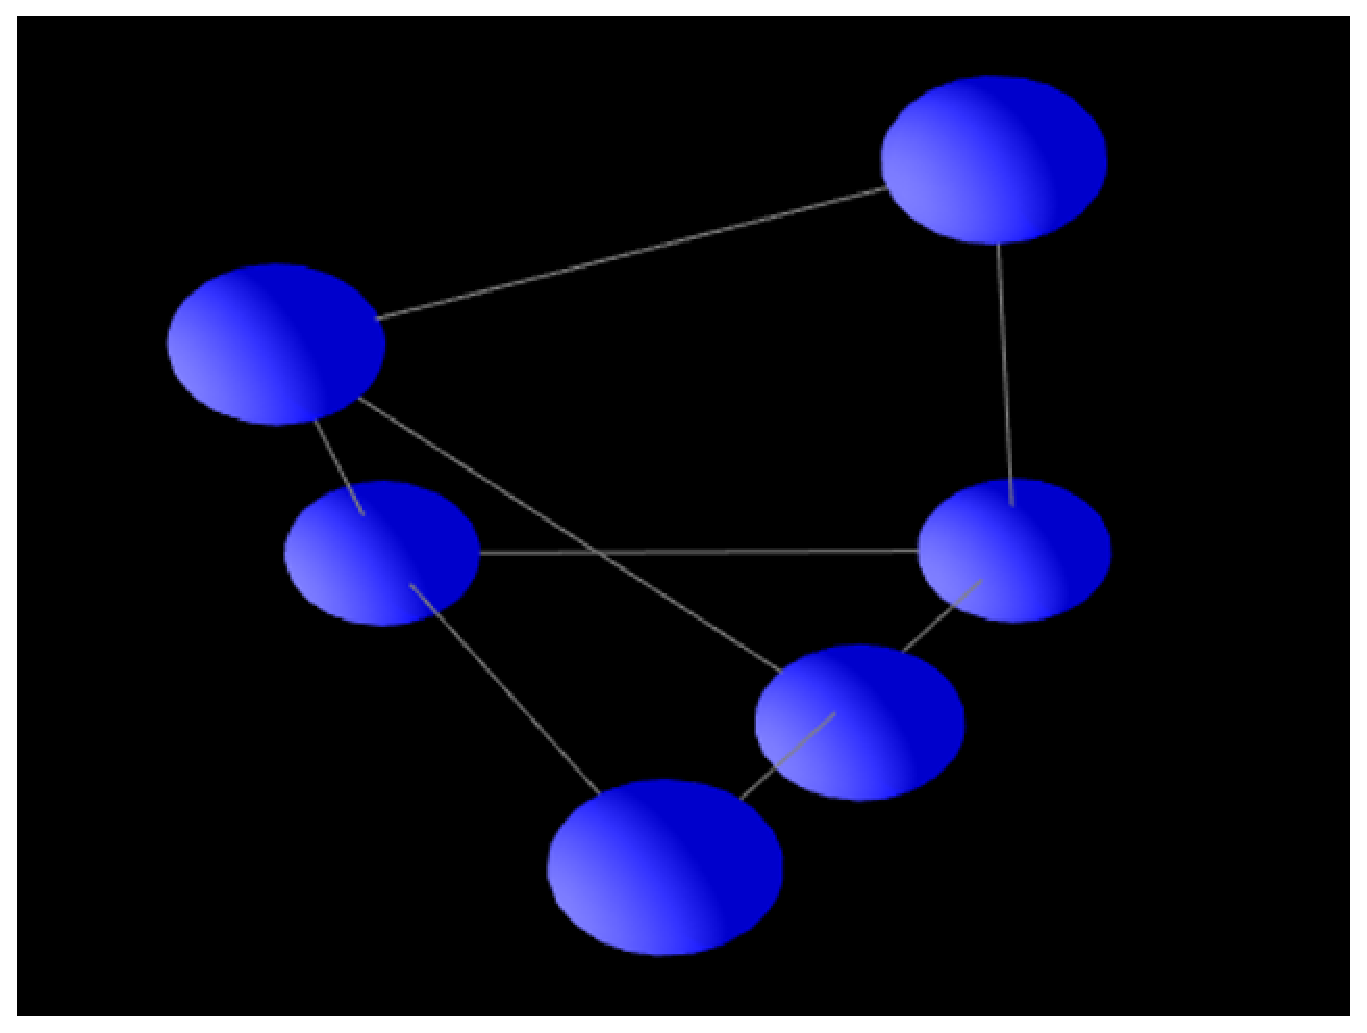
\includegraphics[scale=0.4]{contents/gnode}
  \end{center}
  \caption{Graphe de référence avec nœuds modélisé}
  \label{fig:gnode}
\end{figure}

Maintenant que nous avons un modèle à dessiner pour représenter les nœuds. Pour dessiner chaque nœud dans la boucle de rendu, il nous suffit de faire une translation du repère de la scène vers les coordonnées du nœud courant, de changer ensuite la couleur à projeter, puis de dessiner le modèle 3D correspondant (récupérer à partir du tableau associatif \texttt{ }) au type enum du nœud courant (récuperer à partir du vecteur ayant pour clef l'identifiant du nœud, et le type enum pour valeur). Nous obtenons la figure.~\ref{fig:gnode} représentant le graphe de référence avec une représentation modélisé des nœuds.

%\subsubsection{Problèmes rencontrés}

\begin{figure}[h]
  \begin{center}
    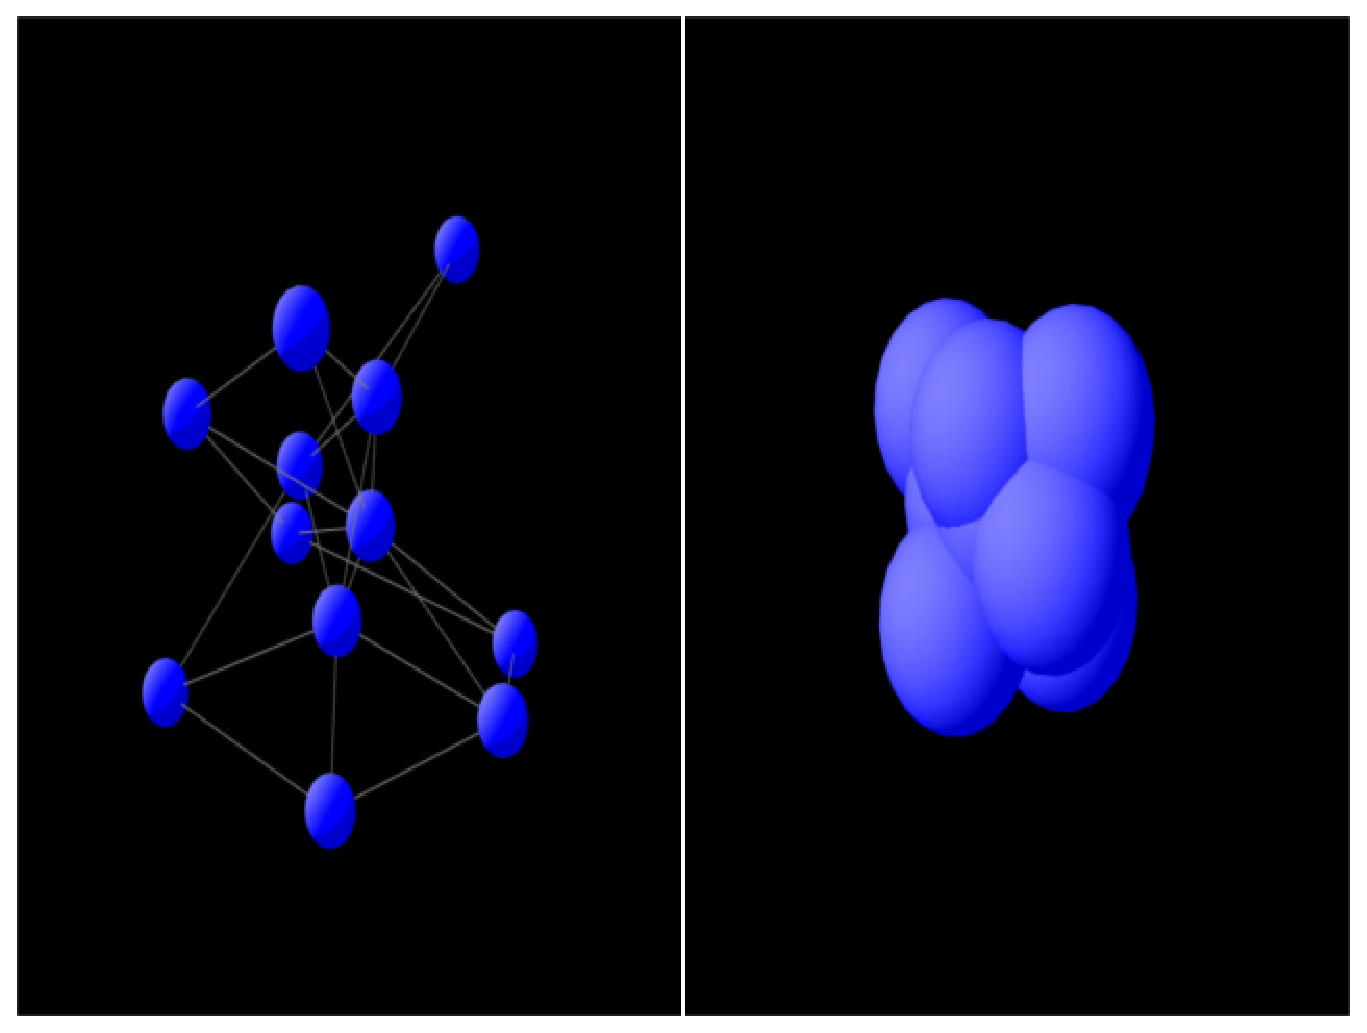
\includegraphics[scale=0.4]{contents/pb2node}
  \end{center}
  \caption{Problème de rendu : dimensions trop grande}
  \label{fig:pb2node}
\end{figure}

\subparagraph{Problème de dimension}

Un problème rencontré est illustré en figure.~\ref{fig:pb2node} partie de droite. Pour illustrer ce problème, nous avons utilisé un autre graphe que celui de référence, puisque sur ce dernier le problème n'est pas visible, car la taille du modèle tombe juste par chance.\\
\texttt{Problème:} Il y a chevauchement des modèles 3D représentatif lorsque le graphe représenté est avec des arêtes courtes et dense.\\
\texttt{Solution:} Utilisation d'une solution proposé par notre encadrant M. Boisson. Nous calculons l'arête ayant la norme euclidienne la plus petite, ceci est tout à fait possible puisque nous connaissons les coordonnées de chaque sommet. Une fois que nous avons la norme minimale \texttt{norme\_min}, nous appliquons une homothétie de telle sorte que le modèle 3D représentant les cellules de données puisse tenir dans un cube de côté $\frac{\texttt{norme\_min}}{3}$. Rappelons que grâce à l'algorithme de placement de nœud utilisé, nous avons une répartition assez harmonieuse dans l'espace dû à la contrainte d'égalité de variance sur les trois axes. Par conséquent, nous n'aurons théoriquement jamais de trop grosses réductions de taille causée par une arête qui serait trop courte par rapport aux autres. Le même graphe rendu avec cette solution appliqué est visible en figure.~\ref{fig:pb2node} sur la partie de gauche.

\subsubsection{Caméra}

Dans cette partie, nous nous occupons de gérer la visualisation de la caméra, ceux-ci seront inspirés du système TrackBall, il s'agit du même système de caméra dans le logiciel \bsc{Google Earth}. Ce système de caméra permettra à l'utilisateur de pouvoir visualiser aisément sa structure de donnée.

La caméra TrackBall consiste à être totalement statique, c'est seulement le contenu de la scène qui va subir des rotations autour des deux axes constituant le plan faisant face à la caméra. Un clique enfoncé suivi d'un mouvement horizontal du curseur fera subir une rotation autour de l'axe verticale (axe \texttt{Y}). Un clique enfoncé suivi d'un mouvement vertical du curseur fera subir une rotation autour de l'axe horizontale (axe \texttt{X}).

Par conséquent, il suffit de sauvegarder la position du curseur sur l'axe X et Y pour la frame courante, puis à la prochaine frame, nous récupérons la position courante du curseur que l'on va soustraire avec la position de la frame précédente que nous avons sauvegardé. Ainsi, nous avons la distance parcourue par le curseur sur l'axe X (\texttt{dist\_parcouru\_X}), et sur l'axe Y (\texttt{dist\_parcouru\_X}), nous pouvons ensuite faire subir une rotation du contenu de la scène grâce à ces deux valeurs. Rotation d'une valeur de \texttt{dist\_parcouru\_X} (éventuellement cœfficienté pour atténuer ou augmenté la sensibilité de la caméra) autour de l'axe \texttt{Y}, puis, une rotation de \texttt{dist\_parcouru\_Y} autour de l'axe \texttt{X}.

La caméra est décrite par son point de position dans le repère universel, un point que la caméra fixe, et le vecteur d'inclinaison de la caméra. Ainsi, pour zoomer, il faut multiplier par un cœfficient inférieur à $1$ les composantes \texttt{x,y,z} du point renseignant la position de la caméra, ainsi le point se rapprochera de l'origine du repère universel, et cela engendrera donc un zoom. Démarche identique pour le dézoom, sauf que nous multiplions par une valeur supérieur à $1$ afin de s'éloigner de l'origine (et donc engendrer un dézoom). Pour le zoom et le dézoom, il s'agit bien de la caméra qui se déplace, pour les rotations, il s'agit de la scène qui subit des rotations.

\subsubsection{Texte}

Cette partie a pour but la visualisation de label de texte pour pouvoir identifier les cellules de données, en effet si nous ne pouvons pas identifier les nœuds du graphe lors de la visualisation, nous ne pourrons que difficilement suivre l'exécution de l'algorithme sur la structure visualisé. Pour cette partie, nous avons utilisé un vertex shader élémentaire, et un fragment shaders gérant les textures avec composante alpha pour la transparence.

Afin d'afficher du texte, nous avons utilisé deux faces triangle rectangle, formant donc un rectangle que nous texturons ensuite avec une texture générée à la volée à partir de \texttt{Qt}. En effet, \texttt{Qt} met à disposition la classe \texttt{QImage} qui est très riche, elle permet entre autres de générer des images bitmap avec canal alpha pour la transparence à partir d'un texte en ASCII, nous pouvons ensuite utiliser cette image pour texturer notre rectangle. On associe le style d'écriture et la couleur du texte dans le tableau associatif associant la structure \texttt{DataNode} au type enum. Le contenu du texte à afficher est simplement le numéro du nœud courant dans notre programme, nous affichons donc tout simplement l'indice d'incrémentation dans notre boucle d'affichage de texte.

Une fois que notre rectangle est texturé avec la texture courante, nous procédons de la même manière que pour les modèles représentant les nœuds. Nous appliquons une translation vers les coordonnées du nœuds courant, puis nous affichons le rectangle texturé.

Ce principe est très présent dans le jeu vidéo, il s'agit de \texttt{sprite}, cette technique peut être utilisé pour animer un personnage en 2D, ou pour certaine interface de menu de configuration, etc. Nous obtenons la figure.~\ref{fig:tnode}

\begin{figure}[h]
  \begin{center}
    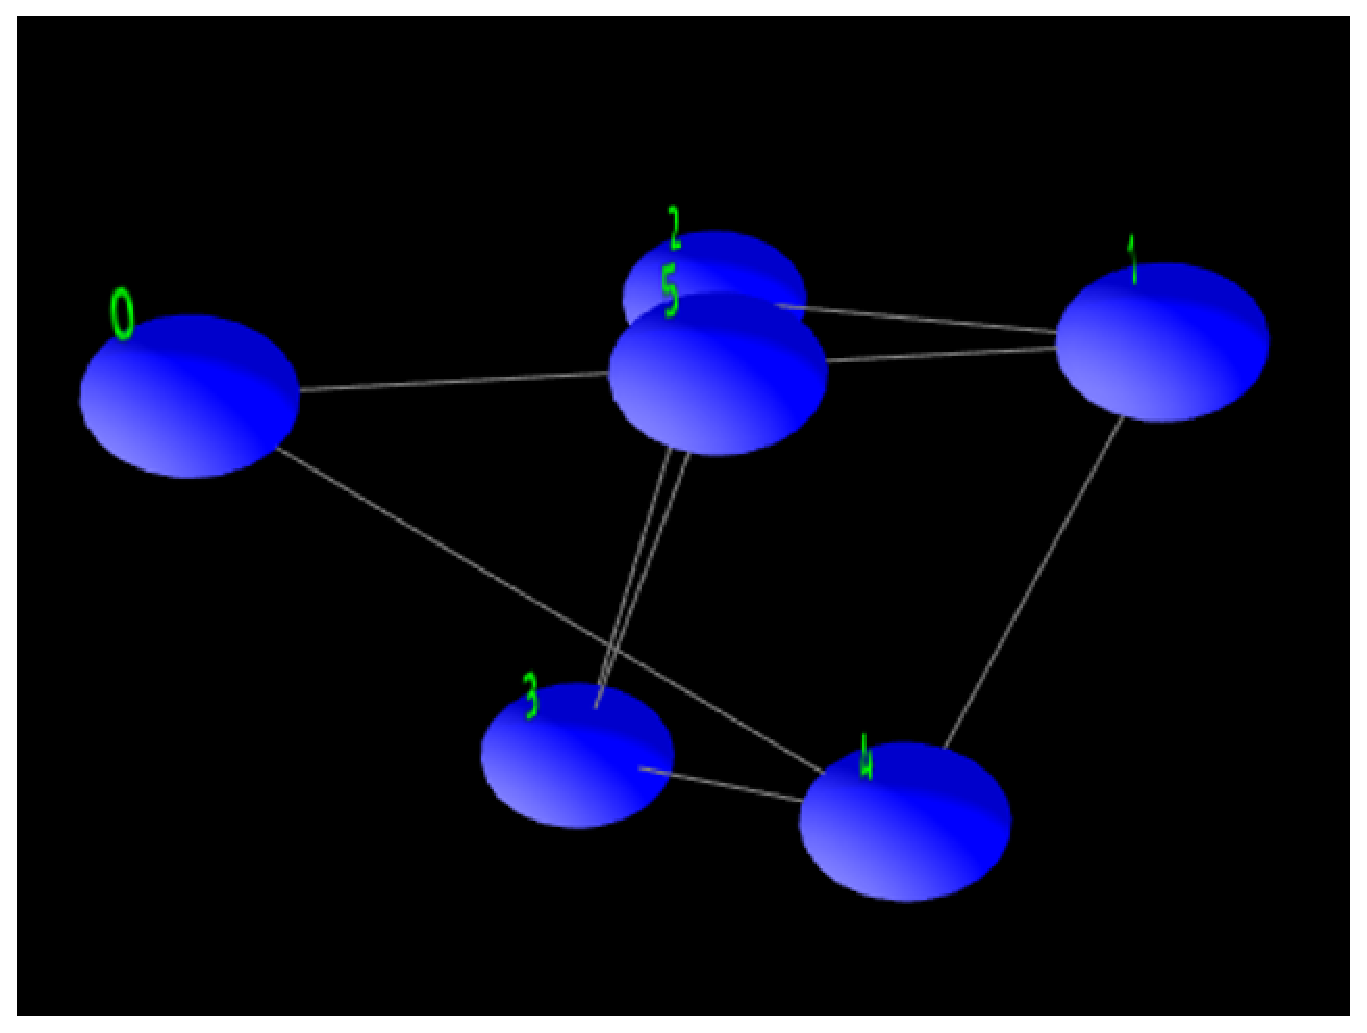
\includegraphics[scale=0.4]{contents/tnode}
  \end{center}
  \caption{Problème de rendu: texte pas toujours face à la caméra}
  \label{fig:tnode}
\end{figure}

Le principal problème de cette approche est que le texte n'est pas toujours face à la caméra comme nous pouvons le voir sur la figure.~\ref{fig:tnode}. En effet, le sprite subit les rotations du contenu de la scène relatif à notre implémentation de caméra TrackBall, rappelons que ce type de caméra est statique, la position de la caméra ne bouge pas, il s'agit du contenu de la scène qui subit les rotations, dont le texte. Nous devons donc faire en sorte que le texte ne subisse pas les rotations nécessaires au fonctionnement de la caméra. Pour cela nous allons utiliser la technique du billboarding.

Cette méthode était utilisée en grande abondance dans le jeu vidéo à l'époque de la \bsc{Nintendo 64} et est encore très utilisé, mais généralement pour d'autres objectifs. Le principal objectif de l'utilisation du billboarding à l'époque de la Nintendo64 était de réduire la complexité des modèles afin de ne pas avoir à gérer trop de données (position de sommets, de placements de texture, etc) pour générer une frame. Par conséquent, il était courant de jouer sur l'illusion. Par exemple, un tronc d'arbre représenté par un rectangle texturé qui tourne autour de lui-même pour toujours faire face à la caméra. Ainsi, au lieu d'avoir un grand nombre de sommets nécessaire à un cylindre, il n'y aura seulement que quatre sommets formant deux triangles texturés avec une texture de tronc d'arbre. Cela réduit donc parfois drastiquement la complexité des modèles lorsque l'on utilise la technique du billboarding dans le cas d'essai d'illusions visuels. Dans Mario Kart 64, cette méthode de billboarding est aussi très utilisé, puisque nous conduisons en réalité des rectangles avec des textures dynamiques faisant toujours face à la caméra, les textures sont modifiés selon les entrées utilisateurs, si l'utilisateur tourne à droite, il suffit de modifier la texture à afficher en conséquence pour y mettre un kart tournant à droite.

\begin{figure}[ht]
  \begin{center}
    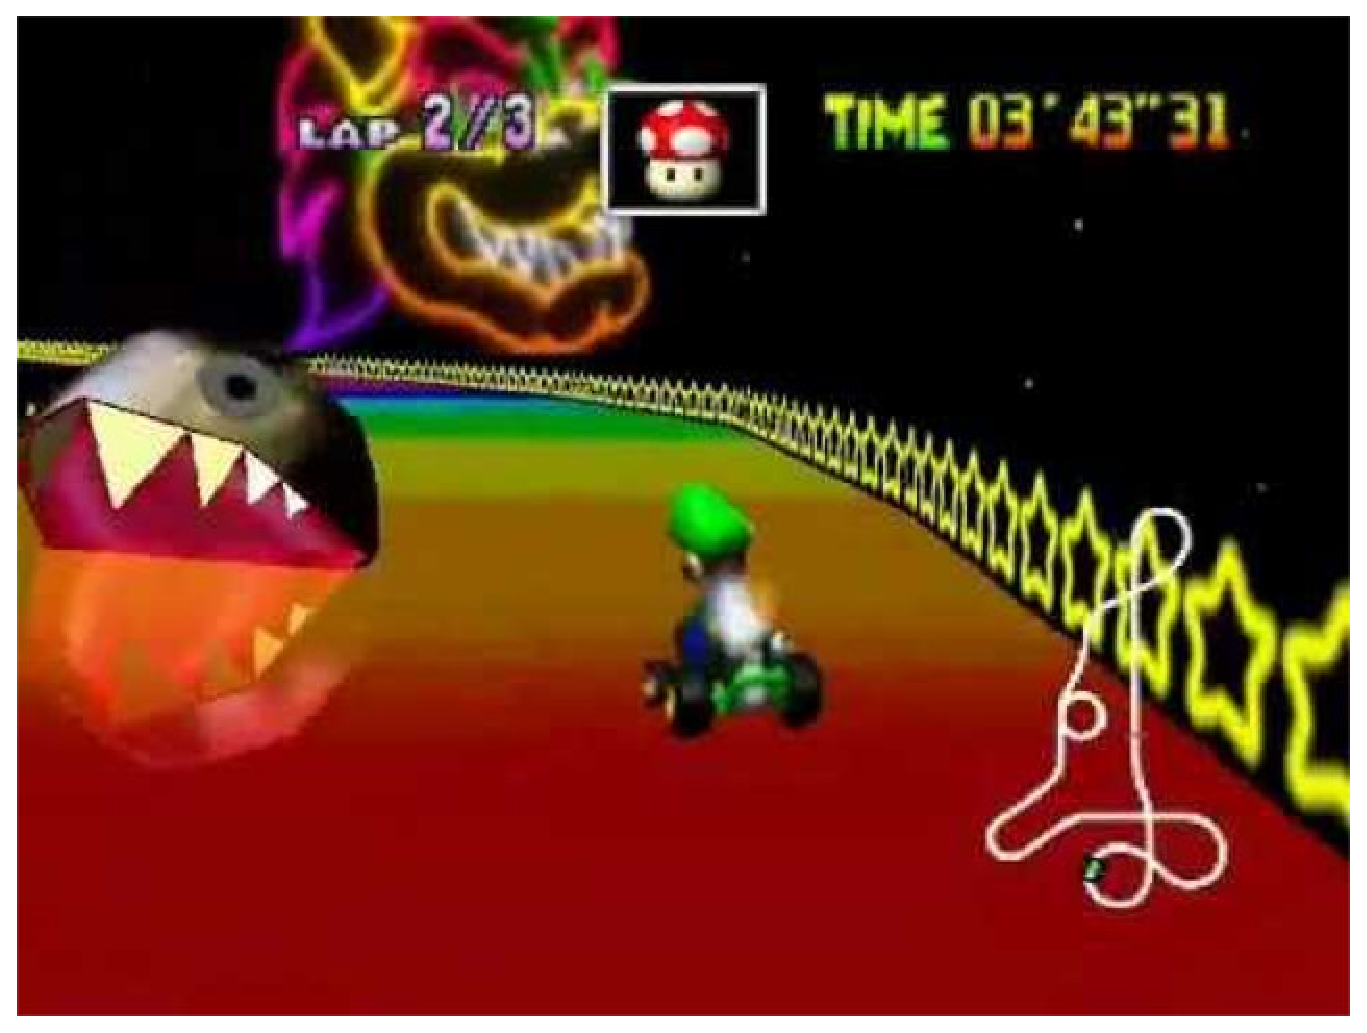
\includegraphics[scale=0.4]{contents/mk64}
  \end{center}
  \caption{Utilisation du billboarding dans \bsc{Mario Kart 64}}
  \label{fig:mk64}
\end{figure}

Actuellement, cette technique est toujours très utilisée, mais rarement en ayant pour objectif d'afficher des sprites faisant face à la caméra, mais plutôt pour qu'un personnage regarde en direction d'un autre personnage lorsque celui-ci s'approche du personnage spectateur, il suffit d'appliquer la même approche, le repère du spectateur doit toujours faire face au personnage en question de la même manière que le texte soit toujours face à la caméra.

La méthode du billboarding est applicable de plusieurs manières, nous utiliserons la manière la plus simple qui nous semble être l'annulation de rotation à partir de modification de valeur dans les matrices de projections et de vue, elle est expliquée en pratique dans \cite{billboard}. En pratique, il suffit simplement de multiplier d'abord la matrice de vue avec la matrice de modèle. Puis de garder en diagonale les valeurs du scale, et enfin de multiplier à gauche par la matrice de projection. Nous obtenons la figure.~\ref{fig:tnode_bb}

\begin{figure}[ht]
  \begin{center}
    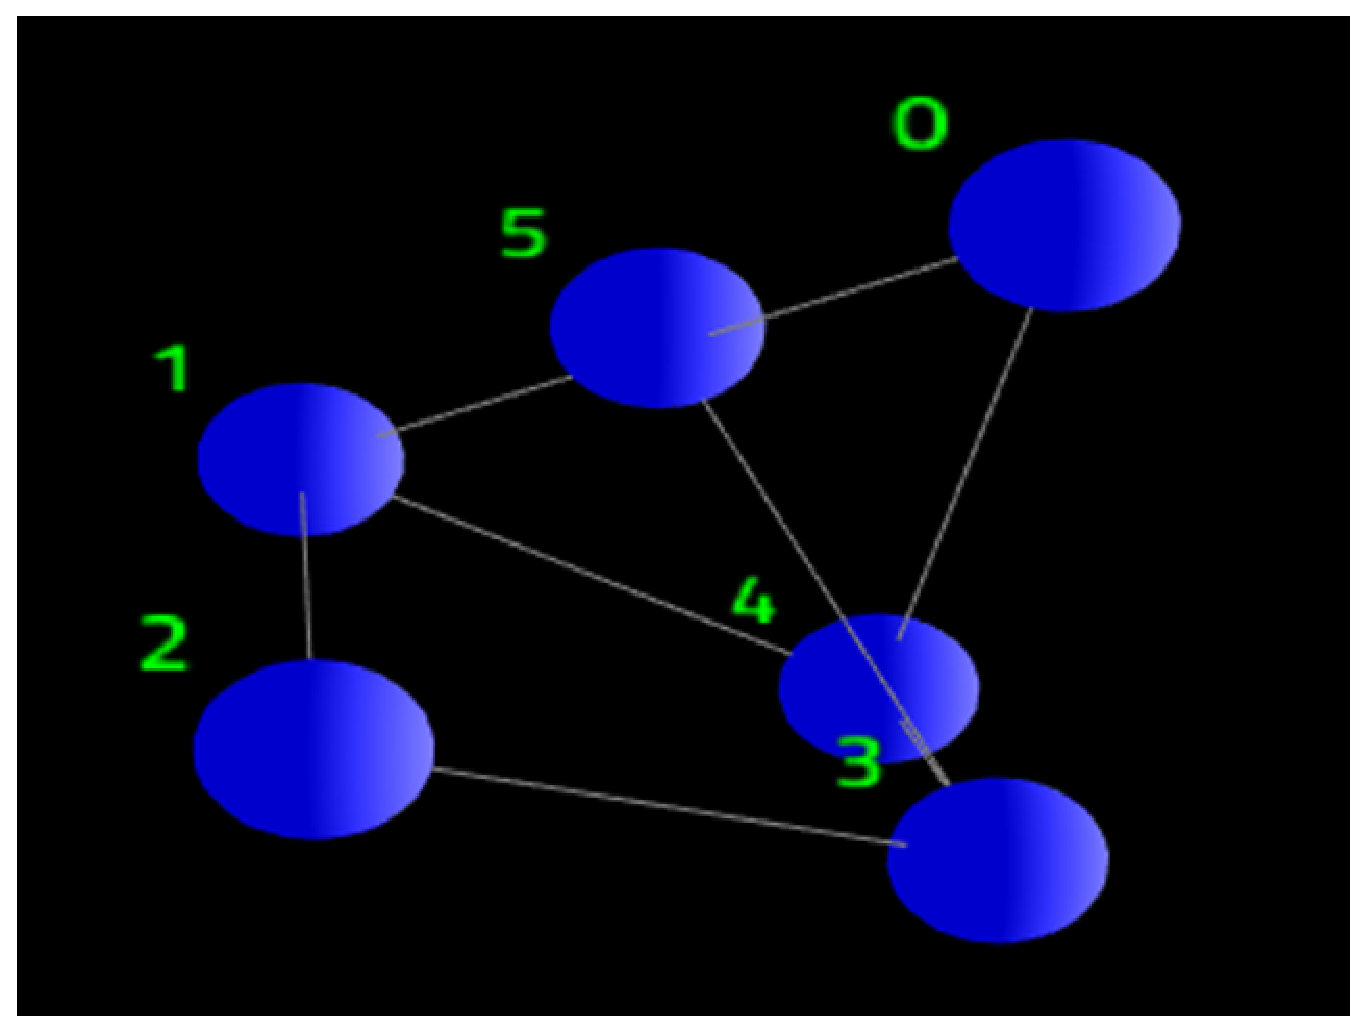
\includegraphics[scale=0.4]{contents/tnode_bb}
  \end{center}
  \caption{Texte avec billboarding}
  \label{fig:tnode_bb}
\end{figure}

\newpage
\section{Conclusions et perspectives}
%TODO: séparé les différents type d'améliorations possibles (logiciel/portabilité/etc)
En conclusion, notre prototype de framework permet une visualisation élementaire d'algorithme sur structure de donnée de graphe. Cette base est assez générique pour pouvoir l'augmentée assez facilement sans à avoir à modifier trop de choses dans la base déjà présente. En effet, il est possible d'ajouter ses propres structures de données, ses propres données de visualisation pour pouvoir ainsi visualiser l'exécution de son algorithme à la manière désiré. Cependant, notre prototype de framework n'a aucune intéractivité lié à l'exécution intrinséque de l'algorithme. L'intéraction présente n'est que lié à la visualisation, et non aux données manipuler par l'algorithme. L'intéraction présente dans ce projet se limite donc à l'implémentation de la caméra manipulable à la souris, et au texte affichable dans le widget dédiée au texte personnalisé.

Nous avons pu apprendre beaucoup de choses grâce à ce projet d'initiation découverte au domaine de la synthèse d'image qui est un domaine qui nous intéresse plus particulièrement. Nous regrettons cependant de ne pas avoir pu mettre davantage en pratique le paradigme de programmation générique de C++ qui est une facette que nous aurions bien aimé mieux maitriser, bien que nous avons pu apprendre certaines spécifités de C++11 comme les fonctions lambdas par exemple.

Plusieurs perspectives d'améliorations sont possibles.
\begin{itemize}
\item augmenter le nombre de structure visualisable dont certaines ont un placement trivial (tableau, liste, etc).
\item Adapter ce programme pour \texttt{OpenGL ES}, afin que le programme soit exécutable sur smartphone et tablettes, ou WebGL pour qu'il soit exécutable sur un navigateur standard.
\item Adapter ce framework en programme éducatif. Exemple: interface avec des questions comme ''quel sera le prochain nœud visité en suivant l'algorithme DFS?''.
\item Améliorer l'interaction, (peut faire partie de l'adaptation à \texttt{OpenGL ES}).
\item Améliorer significativement la gestion de la camera en ayant pour objectif un meilleur suivi, par exemple un zoom progressif sur le nœud visité le plus récent, etc.
\item Utilisation du design pattern CRTP (Curiously Recursiv Template Pattern) qui est un design pattern permettant de supprimer le surcoût de la virtualité grâce à la programmation générique.
\end{itemize}

\section{Remerciements}
Nous remercions l'équipe pédagogique pour avoir accepter de pouvoir proposer un thème de projet qui nous intéressait. Nous remercions aussi M. Boisson pour en avoir fait un sujet de projet très intéressant et de nous avoir aidé à partir de conseils et astuces durant toute la durée de ce projet.

\newpage
\bibliographystyle{alpha}
\bibliography{606_23}

\end{document}
